\documentclass[12pt,a4,twoside]{article}
\usepackage{polyglossia}
\usepackage[style=iso-numeric]{biblatex}
\usepackage[utf8]{inputenc}
\usepackage{amsmath}
\usepackage{graphicx}
\usepackage{float}
\usepackage[margin=2.5cm]{geometry}
\usepackage{hyperref}
\usepackage{enumitem}

\setmainlanguage{english}
\addbibresource{bib/ref.bib}

\def\abstract{
    \section*{\abstractname}
    \markboth{\MakeUppercase{\abstractname}}{}
}
\def\endabstract{\clearpage}

\providecommand{\keywords}[1]
{
    \small	
    \textbf{\textit{Keywords -- }} #1
}

\hypersetup{
    colorlinks = true,
    urlcolor = blue,
    linkcolor = blue,
    citecolor = red
}

\begin{document}

\begin{titlepage}

\newcommand{\HRule}{\rule{\linewidth}{0.1mm}}

\center
 
% ----------------------------------------------------------------------------------------
%	 HEADING SECTIONS
% ----------------------------------------------------------------------------------------


\includegraphics[scale=.75]{graphics/logo-fit-en-cerna.pdf}\\[2cm]
\textsc{\Large Information Security}\\[0.5cm]
\textsc{\large NI-IBE}\\[0.5cm]

% ----------------------------------------------------------------------------------------
%	 TITLE SECTION
% ----------------------------------------------------------------------------------------

\HRule \\[0.4cm]
{ \huge \bfseries Software Development Security}\\[0.4cm]
\HRule \\[1.5cm]
 
% ----------------------------------------------------------------------------------------
%	 AUTHOR SECTION
% ----------------------------------------------------------------------------------------

\begin{minipage}{0.4\textwidth}
\begin{flushleft} \large
\emph{Autor:}\\
Tomáš \textsc{PATRO}\\
\end{flushleft}

\end{minipage}\\[2cm]

% ----------------------------------------------------------------------------------------
%	 DATE SECTION
% ----------------------------------------------------------------------------------------

{\large \today}\\[2cm]

\vfill

\end{titlepage}

\newpage

\begin{abstract}

Software development security is an essential and fundamental part of developing a piece of software. The real-life industry projects' experiences show us that security is often a part of each phase of the Software Development Life Cycle (SDLC).

In this article, we look at the SDLC definition and describe each phase of the process. We put each phase into the context of development security. Based on the knowledge about the SDLC, we look at the three different processes used by the major players in the industry. The aim of these processes is to formalize activities and approaches to develop the software securely. As an addition, in the last section, we talk about the best practices for software development security.\\

\noindent
\keywords{software, security, development, sdlc, process, processes, application, management, risk, best, practices}
\end{abstract}

\tableofcontents
\newpage

\section*{Introduction}
\addcontentsline{toc}{section}{Introduction}

The software engineers pointed their fingers at the inability to handle the computer systems' complexity as early as 1968. It happened during the first software engineering conference organized by NATO. \cite{randell19961968} 

The security during the development very much depends on the complexity of the overall system. The more complex the system is, the more we emphasize the importance of development security. However, the experience from the industry shows us that security during the development is often based on intuition and somewhat incomplete heuristics.

In this article, we will look at the Software Development Life Cycle (SDLC) in the context of the development security. We will also acquaint the reader with two different approaches to enforce a secure development -- security process frameworks and usage of the best practices. Based on the gained information, these approaches show their potential and may apply to a lot of different software projects. However, it is also important to note that these are not the only viable options for development security. There are many other mechanisms on how to ensure development security; we will talk about only two of them.

\newpage

\section{Software Development Life Cycle (SDLC)}
\label{sec:sdlc}

In this section, we will talk about the software development life cycle. It is a fundamental term in software engineering, and it is good first to gain a better knowledge of this process, so we can put it into the context of the development security.

Every controlled process has some form of the life cycle, which determines the particular steps we take from the beginning to the end of the process. If we have a defined process, we can also define the resources and additional information connected to each step of the process. It is not different from the development of a piece of software.

The software development life cycle also defines several steps that determine the process of development of the software. These steps are the application of standard business practices to building software applications. The process is typically divided into six to eight steps. Some project managers may combine, split, or omit some steps, depending on the project's scope. \cite{sdlc_phoenix}

\begin{figure}[h]
\centering
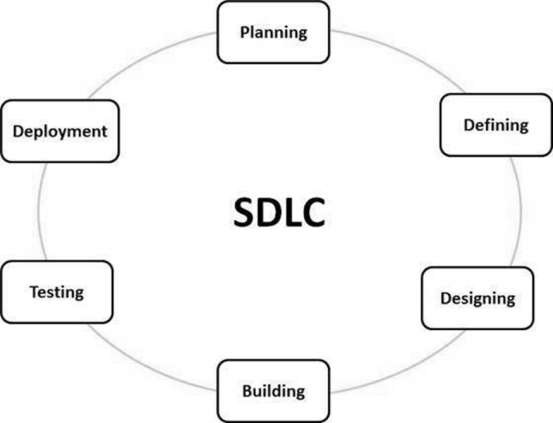
\includegraphics[width=.8\textwidth]{figures/sdlc_stages.jpg}
\caption{A typical SDLC consists of these stages \cite{sdlc_tutorials_point}}
\label{fig:sdlc_stages}
\end{figure}

\subsection{Planning}

Planning is often tightly connected with the requirements analysis. The senior team members often perform it. The inputs mostly come from the customer, sales department, market surveys, and domain experts in the industry. This information is later used to plan the project approach and conduct the feasibility study. \cite{sdlc_tutorials_point}

Another part of the planning may also be quality assurance requirements. These requirements often involve the identification of the risks associated with the project. The risks are often included in the feasibility study's technical part, which may also contain an overview of the security risks. \cite{sdlc_tutorials_point}

\subsection{Defining}

Once the requirements analysis is done, the next step is to clearly and formally document the product requirements, which are later discussed and approved by the customer or the market analysts. There is often a need to redefine these requirements based on customer feedback or feedback from other sources. The redefining can also be connected to the searching for potential security threads and risks. \cite{sdlc_tutorials_point}

\subsection{Designing}

The design involves the architects to come out with the best architecture for the product to be developed. The product of this step is often some form of a design specification. This specification is then reviewed by all important stakeholders and based on various parameters as risk assessment, product robustness, design modularity, etc. \cite{sdlc_tutorials_point}

Some aspects of the design include architecture, user interface, platforms, programming, and communications. The security aspect is also often a part of this step. It defines the measures to be taken to secure the application and can involve things like SSL encryption, password protection, and secure storage of user credentials. \cite{sdlc_phoenix}

\subsection{Building}

In this stage, the actual code is written, and the product is built. Developers must follow the coding guidelines defined by their organization, and programming tools like compilers, interpreters, debuggers, etc., are used to generate the code. The guidelines may include a set of best practices that often help write a better and more secure code. \cite{sdlc_tutorials_point}

The coding process also includes many other tasks. The developers often face tasks like finding and fixing errors and critical glitches. These aspects can often hold up the development process. However, it is also important for the code's overall security to address these issues in the development process. \cite{sdlc_phoenix}

Documentation can also be a guideline of the application's basic features. It can have a form of written documentation like user guides, troubleshooting guides, edge cases analysis, etc. \cite{sdlc_phoenix}

\subsection{Testing}

This step is often a subset of all the stages in the SDLC. However, this step refers to the testing only stage of the product where we detect products' security issues, bugs, glitches, and other types of defects. The defects need to be addressed and reprogrammed accordingly. This step should end only if the product reaches the company's quality standards. \cite{sdlc_tutorials_point}

Much of the testing can also be automated. This also includes security testing like static or dynamic code analysis, etc. \cite{sdlc_phoenix}

\subsection{Deployment}

The deployment involves a formal release of the product in the appropriate market. Sometimes the product deployment happens in stages as per the business strategy of the company. The product may be first released in a limited segment and tested in the real business environment (user acceptance testing). Based on the feedback, the product may be adjusted accordingly. There is also a space for finding potential bugs or security issues not detected by the testing phase. \cite{sdlc_tutorials_point}

Many companies prefer to automate the deployment phase. The automation may be complex and needs to be finely orchestrated not to bring security defects to the deployment process. \cite{sdlc_phoenix}

\subsection{Operation and Maintenance}

At this point, the product is developed and used in the field. However, the operation and maintenance phase is still important. In this step, the users discover and report bugs and security issues that weren't found during coding and testing. These errors need to be resolved, which may spawn new development cycles. \cite{sdlc_phoenix}

Often, a part of this phase is also some form of service-level agreement (SLA) between the customer and provider. This agreement documents what services the provider will furnish and defines the service standards the provider is obligated to meet. This may also include security measures that will be taken by the service provider are defined. Typically, this includes the drafting and consensus on antipoaching, IT security, and nondisclosure agreements. \cite{sla}

\subsection{SDLC Summary}

Based on the steps described above, we may conclude that development security is included in all the SDLC steps (phases). We can ask ourselves the question of how to approach security in the development process. There may be many answers to this question. One possible solution may be to define a set of standards/processes that should be followed throughout the SDLC.

\section{Secure Software Development Processes}
\label{sec:ssdp}

In this section, we will look at the three processes which are used to ensure the security during the SDLC. The focus is put on three forefront representatives, namely Microsoft's \textit{Security Development Lifecycle} (SDL) \cite{microsoft_sdl}, OWASP’s \textit{Comprehensive, Lightweight Application Security Process} (CLASP) \cite{owasp}, and McGraw' \textit{Touchpoints} \cite{mcgraw2004software}.

In Section \ref{sec:sdlc} we stated that the security issues are present in all phases of the SDLC. However, the construction of secure software is still largely a matter of guidelines, best practices, and undocumented expert knowledge in many companies. \cite{on_secure_software}

Several advances have been made in the definition of the process for secure software development by the major players in the field like Microsoft or OWASP. The information about the processes are taken from the \textit{Bart De Win's} paper \textit{On the secure software development process: CLASP, SDL and Touchpoints compared} \cite{on_secure_software}.

\subsection{Security Development Lifecycle (SDL) \cite{on_secure_software}}

In 2002, Microsoft made a commitment to follow the so-called ``trustworthy computing'' principle. As a result, the company defined the \textit{Security Development Lifecycle (SDL)}. SDL is a process definition that is composed of a set of activities, which complement Microsoft's development process. These activities are particularly aimed to address security issues during the development process. The following aspects characterize the process:

\begin{enumerate}
    \item Security as a supporting quality
    \item Well-defined process
    \item Good guidance
    \item Management perspective
\end{enumerate}

\begin{figure}[h]
\centering
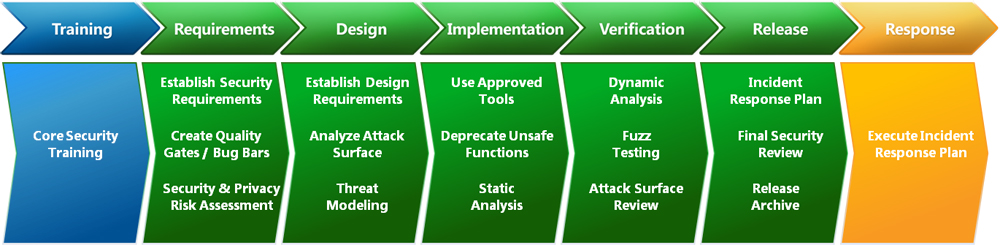
\includegraphics[width=1\textwidth]{figures/sdl_steps.jpg}
\caption{The seven phases of the Security Development Lifecycle Process. \cite{sdl_wiki}}
\label{fig:sdl_phases}
\end{figure}

\subsubsection{Security as Supporting Quality}

The primary goal of SDL is to function as a supportive add-on to the software construction process. It reaches this functionality by increasing the quality of functionality-driven software. This is done by improving its security approach.

Security activities are most often related to functionality-based construction activities. For example, threat modeling starts from architectural dependencies with the external systems. However, the architecture itself could, in fact, reduce such threats in the first place. The SDL defines many similar approaches to enrich the quality of the development security.

\subsubsection{Well-defined Process}

From Figure \ref{fig:sdl_phases}, we can see that SDL is well-organized into the phases similar to the SDLC described in Section \ref{sec:sdlc}. Although the stages are security-specific, it is straightforward to map them to standard software development phases -- in the section \ref{sec:sdlc} we concluded that security is often included in all steps of the SDLC.

Furthermore, several activities have continuous characteristics. This includes threat modeling and education. Thus, the SDL process incorporates support for revising and improving intermediate results.

\subsubsection{Good Guidance}

SDL achieves good guidance by specifying the method that must be used to execute activities.  On average, these specifications are concrete and often somewhat pragmatic. For example, the attack surface reduction is guided by a flow chart. Another example can be threat modeling, which is described as a set of sub-processes. As a result, the execution of an activity is quite achievable, even for less experienced people.

\subsubsection{Management Perspective}

Often in the companies, we can observe that security as quality has to be managed in order to be realized in practice. SDL takes a management perspective for the description of many activities. This is a very convenient feature given the inherent complexity of the security.

\subsection{Comprehensive, Lightweight Application Security Process (CLASP) \cite{on_secure_software}}

CLASP is a \textit{lightweight} process for building secure software. It consists of 24 top-level activities, which are general enough to be tailored to the development process in progress. Some of the key features include:

\begin{enumerate}
    \item Security at the center stage
    \item Limited structure
    \item Role-based
    \item Rich in resources
\end{enumerate}

\begin{figure}[h]
\centering
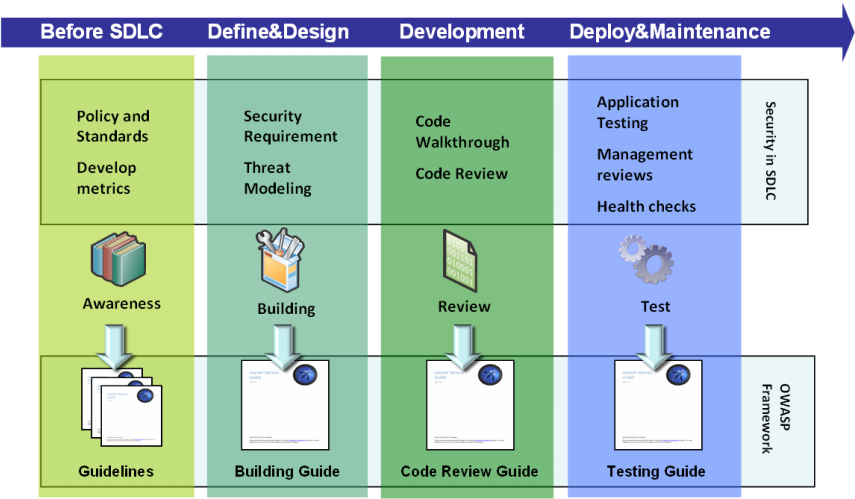
\includegraphics[width=1\textwidth]{figures/owasp_clasp.png}
\caption{SDLC \& OWASP Guidelines. \cite{owasp_clasp}}
\label{fig:sdlc_owasp}
\end{figure}

\subsubsection{Security at Center Stage}

As shown in Figure \ref{fig:sdlc_owasp}, the CLASP framework is mainly proposed for the construction of software in which security takes a central role. The set of activities is fairly broad since they are defined and conceived primarily from a security-theoretical perspective.

\subsubsection{Limited Structure}

CLASP framework offers a certain level of flexibility. It is achieved by the independence of the activities that have to be integrated into the development process and its operating environment. It is up to a particular company to choose the activities to be executed and choose the order of execution. Moreover, the execution frequency is specified per individual activity. The coordination and synchronization of the activities may thus not be straightforward. Besides, the CLASP framework defines two road maps ( ``legacy'' and ``greenfield''), which give some guidance on how to combine the activities into a coherent and ordered set.

\subsubsection{Role-based}

We already mentioned activities, which are the building blocks of the CLASP. The framework also consists of the roles responsible for the finalization and the quality of the results of an activity. These roles can also have a direct impact on the security approach. Roles are used as an additional perspective to structure the set of activities.

\subsubsection{Rich in Resources}

CLASP provides and an extensive set of security resources used as support in the implementation of the activities. For example, one of the resources is a list of 104 known security vulnerabilities in application source code.

\subsection{Touchpoints \cite{on_secure_software}}

Let's introduce Gary McGraw, the author of the \textit{Seven Touchpoints for Software Security}, first:\\

\textit{``Gary McGraw is the CTO of \textit{Cigital, Inc.}, a software security and quality consulting firm providing services to some of the world's best-known companies for a decade. Dr. McGraw is a globally-recognized authority on software security-featured frequently as a keynote speaker at events coast-to-coast as well as internationally.''} \cite{mcgraw_software_security}

Touchpoints describe a set of security best practices that come from the extensive industrial experience of McGraw. The best practices (activities) are grouped together in seven so-called touchpoints. Some of the aspects of Touchpoints include:

\begin{enumerate}
    \item Risk management
    \item Black vs. white
    \item Flexibility
    \item Examples
    \item Resources
\end{enumerate}

\begin{figure}[h]
\centering
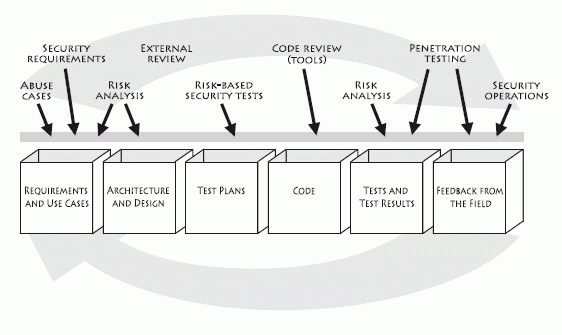
\includegraphics[width=1\textwidth]{figures/touchpoints.png}
\caption{Seven touchpoints (best practices) of software security. \cite{mcgraw_software_security}}
\label{fig:touchpoints}
\end{figure}

\subsubsection{Risk management}

Risk management is an important part of software security. Touchpoints acknowledge its importance and try to bridge the gap by elaborating the \textit{Risk Management Framework (RMF)} that supports the Touchpoints activities.

\subsubsection{Black vs. white}

Touchpoints come with a mix of black-hat and white-hat activities. Both types are equal in the means of necessity. Black-hat activities aim for attacks, exploits, and breaking software -- penetration testing. On the other hand, white-hat activities are more constructive in nature. They cover design, control, and functionality -- code review.

\subsubsection{Flexibility}

Since the Touchpoints are formalized in the form of best practices, we can tailor them and use them for software that already undergoes development. Besides, the documentation provides prioritization of different touchpoints. Thus, the companies are able to gradually introduce the touchpoints, starting from the most important ones.

\subsubsection{Examples}

Touchpoints bring lots of examples. For example, while describing the abuse cases, there is an example giving the reader a good feel about what they might look like in a particular situation.

\subsubsection{Resources}

Part of the Touchpoints is dedicated to security knowledge where resources are part of it. The resources further aid the execution of activities. Touchpoints provide references to resources and explain how to use them. For example, attack patterns are provided in order to be used in the elicitation of abuse cases.

\subsection{Processes Conclusions}

There is always a question about which process or methodology to use for your project. The answer is that it very much depends on a particular situation. We described three widely used processes and their main characteristics. If you want to know more and read about the comparison of these three processes, we recommend to read \textit{Bart De Win's} paper \textit{On the secure software development process: CLASP, SDL and Touchpoints compared} \cite{on_secure_software}. De Win and his colleagues summarized and compared these processes looking at a lot of different characteristics from education and awareness through release and deployment to support.

\section{Software Development Security Best Practices}
\label{sec:best_practices}

This last section will look at a subset of the practical best practices for secure software development. We will look at the list of the best practices described by \textit{Ansar-Ul-Haque Yasar}, and his colleagues in the paper \textit{Best practices for software security: An overview} \cite{security_best_practices}. Yasar et al. made a list of the best practices from the different sources. Yasar et al. also state the following:\\

\textit{``Software security spread covers the whole Software Development Life Cycle phases. Each of the phases should be carefully observed for building secure software.''\\}

We can relate to this statement as we described it in Section \ref{sec:sdlc}. Yasar et al. chose three example sets of best practices and classified them based on the phases of the SDLC.

\subsection{Best Practices -- Set 1}

Davis et al. proposed the first set in the paper \textit{Processes for producing secure software} \cite{davis_secure_software}. The set is composed of these practices, which should be executed in this order:

\begin{enumerate}[noitemsep]
    \item Abuse cases
    \item Security requirements
    \item Risk analysis
    \item External review
    \item Risk-based security tests
    \item Static analysis (tools)
    \item Risk analysis
    \item Penetration testing
    \item Security breaks
\end{enumerate}

\begin{figure}[h]
\centering
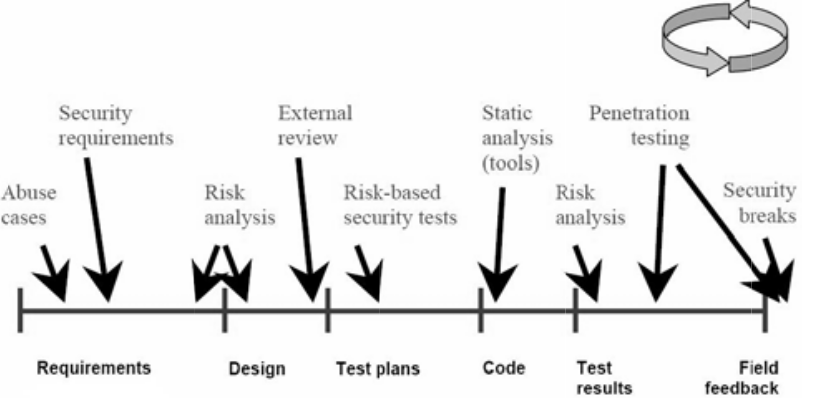
\includegraphics[width=.8\textwidth]{figures/best_practices.png}
\caption{Best practices for the software security represented by software artifacts. \cite{davis_secure_software}}
\label{fig:best_practices}
\end{figure}

The SDLC is divided into the so-called self-explanatory subgroups, i.e., software artifacts describing the activities performed during the phases. The practices mentioned above are afterward mapped to these artifacts.

\subsection{Best Practices -- Set 2 \& 3}

The other two sets are rather composed of straightforward recommendations. We will list them and add a simple explanation to each of them. The second set is proposed by \textit{Razvan Peteanu} in the paper \textit{Best Practices for Secure Development} \cite{razvan_best_practices}. Peteanu proposed high-level best practices for secure development:

\begin{enumerate}
    \item \textbf{Relevancy and weakest links} -- protect the related information and secure the places which may be more prone to attacks.
    \item \textbf{Clarity} -- we should define every aspect of the solution we provide.
    \item \textbf{Quality} -- the quality of security should be evenly maintained with the quality of the overall product.
    \item \textbf{Involve all stakeholders} -- all relevant stakeholders should be involved in the security process (level of involvement should also be defined).
    \item \textbf{Technology processes} -- the processes are related to each other, and there should be a technology able to invoke them.
    \item \textbf{Fail safe operation} -- the product should be able to recover from the errors.
    \item \textbf{Defense in depth} -- we should be able to implement defensive mechanisms in a multi-layered environment.
    \item \textbf{Principle of appropriate privileges} -- everyone should be given privileges to operate the system accordingly considering the development phase and not only the final product.
    \item \textbf{Interacting with users} -- related to the user testing phase. The users often find bugs in the product, and we should address these findings.
    \item \textbf{Trust boundaries} -- we should define the trust boundaries to enforce a reliable security mechanism. For example, we can define a trusted computing base or a trusted path.
    \item \textbf{Third-party software} -- at some point, we may use a third-party software. We should always be cautious when using vendors and potentially also test this software.
    \item \textbf{Manipulation of sensitive data} -- this manipulation should be handled with proper care, and its security should be our top priority.
    \item \textbf{Attack first on paper} -- if possible, it is a good recommendation to try breaking the security architecture during the design phase.
    \item \textbf{Think ``outside of the box''} -- an important concept which tells us to always look for alternative approaches in points of views when testing and trying to break the product.
    \item \textbf{Be humble} -- in the terms when we should continue improving the product even after the release.
    \item \textbf{Declarative vs. programmatic} -- this is the most ``technical'' best practice. It tells us that security should be enforced in the programming either during the execution or outside the program control.
    \item \textbf{Reviews are your best allies} -- also related to the programming. Code reviews should be an essential part of the coding process.
\end{enumerate}

The third and last set is proposed by \textit{David A. Wheeler} in the article \textit{Secure programming for Linux and Unix HOWTO}. This set is the most technical one and aimed mainly for the coding part:

\begin{enumerate}
    \item \textbf{Validate all input} -- every external and internal input to the system should be carefully handled.
    \item \textbf{Avoid buffer overflow} -- we should be careful when working with data structures and not cause stack or heap overflow problems.
    \item \textbf{Secure the interface} -- we should design the interface simple enough to understand it easily.
    \item \textbf{Separate data and control} -- illegal or invalid execution may lead to the loss of important data.
    \item \textbf{Minimize privileges} -- we should carefully consider every permissions/privileges assignment and properly design the policies.
    \item \textbf{Minimize the functionality of a component} -- it is easier to find and fix possible security flaws in a system composed of smaller components than in a monolithic system.
    \item \textbf{Configure safely and user safe defaults} -- we should make the initial system safe as it eases the potential reconfiguration in the future.
    \item \textbf{Load initialization values safely} -- the system often loads these values to set the defaults. It relates to the previous point.
    \item \textbf{Fail safe} -- we should always define a straightforward and safe recovery process from an error.
    \item \textbf{Avoid race conditions} -- multi-threading and multi-processing should be handled carefully by the experienced developers.
    \item \textbf{Trust only trustworthy channels} -- always evaluate if the source of data is reliable and trustworthy.
    \item \textbf{Setup a trusted path} -- always evaluate a process path and look for the possible sources of errors to avoid the leakage of secure information.
    \item \textbf{User internal consistency} -- this refers to the usage of coding standards and application of company policies during the development process.
    \item \textbf{Self-limit resources} -- as abnormal termination may loose some information.
    \item \textbf{Prevent cross-site malicious content} -- avoid data from unreliable sources which may lead to the leakage of other users' data.
    \item \textbf{Foil semantic attacks} -- implement procedures to prevent social engineering on your users like phishing, etc.
    \item \textbf{Be careful with data types} -- many bugs and security flaws are caused by invalid usage of data types.
    \item \textbf{Carefully callout to other resources} -- some resources like library routines may require some additional system information to operate.
    \item \textbf{Send information back judiciously} -- minimize feedback for unreliable users.
\end{enumerate}

The best practices we summarized in the article can be used as a guideline or a checkbox. The advantage of these recommendations is their flexibility and freedom to adapt them to a particular case. Based on the project's complexity and scope, you can use them as an addition to your security process framework or as a core guideline for your development process.

\newpage

\section*{Conclusion}
\addcontentsline{toc}{section}{Conclusion}

In the article, we first defined, in Section \ref{sec:sdlc}, the \textit{Software Development Life Cycle (SDLC)} as one of the fundamental parts of software engineering. We looked at the different steps (phases) of the cycle and briefly put them into the software development security context.

The SDLC description aimed to acquire the reader with the life of the software and its different phases. This section's outcome should be the question of how to ensure the security of development in all phases of the SDLC.

We addressed the question from the first section in the second one where we described three different security processes used in the software development, namely Microsoft's \textit{Security Development Lifecycle} (SDL) \cite{microsoft_sdl}, OWASP’s \textit{Comprehensive, Lightweight Application Security Process} (CLASP) \cite{owasp}, and McGraw' \textit{Touchpoints} \cite{mcgraw2004software}.

In Section \ref{sec:ssdp}, we also described each of the processes' key characteristics and features. In Section \ref{sec:best_practices} we presented three different sets of security best practices. Each set looked at the security from a different level of abstraction. The article's overall purpose was to acquaint the user with the possible ways to ensure security during the development -- using the security process frameworks, security best practices, or combining them.

\newpage
\printbibliography
\addcontentsline{toc}{section}{References}

\end{document}
